\documentclass[11pt,a4paper,twocolumn]{article}
\usepackage[utf8]{inputenc}
\usepackage[T1]{fontenc}
\usepackage{lmodern}
\usepackage{amsmath,amssymb,amsthm}
\usepackage{graphicx}
\usepackage{hyperref}
\usepackage{geometry}
\usepackage{booktabs}
\usepackage{siunitx}
\usepackage{natbib}
\usepackage[protrusion=true,expansion=false]{microtype}
\usepackage[turkish,english]{babel}
\usepackage{authblk}
\usepackage{placeins}
\geometry{margin=2.5cm}

\title{Makroskopik Zaman Genişlemesi Üzerine Birleşik Fizibilite Sınırları:\\Cihaz Ölçeğinde Altı Klasik-GR Mekanizmasının Karşılaştırmalı Analizi}

\author{Erdem Esa\thanks{Corresponding author.}\\ \small Independent Researcher\\ \small \texttt{erdem.esa.71@gmail.com}}

\date{\today}

\begin{document}
\maketitle
\selectlanguage{turkish}
\begin{abstract}
Bu \c{c}al\i{}\c{s}mada, laboratuvar \"ol\c{c}e\u{g}inde makroskopik
zaman geni\c{s}lemesi veya kapal\i{} zaman benzeri e\u{g}riler
(CTC) \"uretmek i\c{c}in \"onerilen alt\i{} fiziksel mekanizma
birle\c{s}ik bir say\i{}sal ve analitik \c{c}er\c{c}evede
incelenmi\c{s}tir: (i) elektromanyetik alan konfig\"urasyonlar\i{},
(ii) Kerr \c{c}er\c{c}eve s\"ur\"uklenmesi, (iii) Tipler d\"onen
silindirleri, (iv) Morris--Thorne solucan delikleri, (v) Alcubierre
b\"uk\"um s\"ur\"uc\"uleri ve (vi) G\"odel d\"onen evreni.
Elektromanyetik durum i\c{c}in, sonlu-telli Biot--Savart kaynak
modeli, tam elektromanyetik enerji-momentum tens\"or\"u ve
lineerle\c{s}tirilmi\c{s} Einstein denklemleri i\c{c}in eksenel
simetrik sonlu fark Poisson \c{c}\"oz\"uc\"us\"un\"u birle\c{s}tiren
ilk-ilkelerden t\"uretilmi\c{s} bir boru hatt\i{} geli\c{s}tirdik.
Di\u{g}er be\c{s} mekanizma i\c{c}in kapal\i{} formda
fizibilite s\i{}n\i{}rlar\i{} t\"urettik. Alt\i{} mekanizman\i{}n
tamam\i{}, cihaz \"ol\c{c}e\u{g}inin $10^{20}$ ile $10^{49}$ kat\i{}
aras\i{}nda kaynak gerektirmektedir. Fiziksel olarak izin verilen
en yak\i{}n mekanizma (elektromanyetik), h\^al\^a magnetar
\"ol\c{c}e\u{g}indeki ak\i{}mlar\i{} a\c{s}an $\sim 10^{22}$~A
ak\i{}m gerektirmektedir. Hi\c{c}bir m\"uhendislik iyile\c{s}tirmesi
bu bo\c{s}lu\u{g}u kapatamaz. Sonu\c{c} olarak, klasik genel
g\"orelilik ile tutarl\i{} hi\c{c}bir mekanizman\i{}n cihaz
\"ol\c{c}e\u{g}inde makroskopik zaman geni\c{s}lemesi i\c{c}in
eri\c{s}ilebilir olmad\i{}\u{g}\i{}n\i{} g\"osteriyoruz.

\end{abstract}


\section{Giriş}
\label{sec:intro}

Genel görelilik çerçevesinde zaman yolculuğu olasılığı, Gödel'in
1949'da kapalı zaman benzeri eğriler (CTC) içeren dönen-evren
çözümünü keşfetmesinden bu yana sürekli ilgi görmüştür
\citep{Godel1949}. Sonraki çalışmalar birkaç ek CTC-barındıran çözüm
tanımladı: Tipler'in dönen silindiri \citep{Tipler1974},
Morris--Thorne geçilebilir solucan deliği \citep{MorrisThorne1988}
ve yeterli spine sahip Kerr karadelikleri \citep{Kerr1963}. Bu
çözümler matematiksel olarak tutarlı olsalar da, gerçekleştirilmeleri
ya sonsuz uzaysal boyut, ya negatif enerji yoğunluklu egzotik madde,
ya da astrofiziksel kütle ölçekleri gerektirir.

Paralel bir araştırma hattı, elektromanyetik alanlar yoluyla CTC
veya makroskopik zaman genişlemesi indükleme olasılığını
araştırmıştır. Elektromanyetik alanlar enerji ve momentum taşır ve
Einstein denklemleri aracılığıyla ilke olarak uzay-zamanı
eğmelidir. Popüler literatürdeki birkaç öneri, laboratuvar ölçeğinde
cihazlar içindeki rezonans elektromanyetik konfigürasyonların
ölçülebilir zamansal etkiler üretmek için yeterli eğrilik
üretebileceğini öne sürmektedir.

Bununla birlikte, bilgimiz dahilinde, elektromanyetik kaynaklı zaman
genişlemesi için sistematik bir cihaz ölçeğinde fizibilite çalışması
mevcut değildir ve bilinen kütleçekimsel mekanizmalara karşı
karşılaştırmalı sınırlar birleşik bir çerçevede derlenmemiştir.

\paragraph{Katkımız.} Bu boşluğu üç özgül katkıyla ele alıyoruz:

\begin{enumerate}
\item Kompakt bir elektromanyetik kaynağı (sonlu-telli bobin dizisi)
      enerji-momentum tensörü üzerinden bir metrik pertürbasyonu
      $h_{\mu\nu}$'ye eşleyen, doğrulanmış eksenel simetrik bir
      Poisson çözücüsü kullanan ilk-ilkelerden bir sayısal boru hattı
      geliştiriyoruz.
\item Beş ek mekanizma için kapalı formda fizibilite sınırlarını
      türetip tablolaştırıyoruz: Kerr çerçeve sürüklenmesi, Tipler
      silindirleri, Morris--Thorne solucan delikleri, Alcubierre
      büküm sürücüleri ve Gödel evreni.
\item Altı mekanizmanın tamamını ortak bir enerji-yoğunluğu-eşdeğeri
      metriğe dönüştürüyoruz ve gereken kaynakların cihaz ölçeğinde
      fizibilite sınırının $10^{20}$ ile $10^{49}$ katı arasında
      yattığını gösteriyoruz.
\end{enumerate}

\paragraph{Kapsam ve sınırlamalar.} Tamamen klasik elektromanyetizma
ile çiftlenmiş klasik genel görelilik çerçevesinde çalışıyoruz.
Yarı-klasik veya kuantum-kütleçekim etkilerini ele almıyoruz.
Amacımız \emph{fizibilite sınırlaması}dır: mevcut ve öngörülebilir
teknolojinin herhangi bir makroskopik zamansal etkinin eşiğinden ne
kadar uzakta olduğunu nicelikselleştirmek.

\paragraph{Düzenleme.} Bölüm~\ref{sec:method} elektromanyetik boru
hattını tanımlar. Bölüm~\ref{sec:results} sayısal sonuçları sunar.
Bölüm~\ref{sec:discussion} fiziksel yorumu tartışır.
Bölüm~\ref{sec:conclusion} sonuçlarımızı özetler.

\section{Yöntem}
\label{sec:method}

\subsection{Elektromanyetik boru hattı}
\label{subsec:em}

Elektromanyetik boru hattımız dört aşamadan oluşur.

\paragraph{Kaynak modeli.} Cihaz bobinlerini, segmentlere ayrılmış
sonlu-kalınlıkta filamentli teller olarak modelliyoruz. Biot--Savart
yasası herhangi bir gözlem noktasındaki manyetik alanı verir:
\begin{equation}
\mathbf{B}(\mathbf{x}) = \frac{\mu_0 I}{4\pi} \sum_i
\frac{d\mathbf{l}_i \times (\mathbf{x} - \mathbf{x}_i)}
{|\mathbf{x} - \mathbf{x}_i|^3}
\end{equation}
burada $\mathbf{x}_i$ ve $d\mathbf{l}_i$ segment orta noktası ve
diferansiyel vektördür. Dört geometri (solenoid, toroid, ters-dönen
helisel çift, hibrid) için sonlu-tel ayrıklaştırması, tek bir
halkanın analitik eksen-üzeri formülüne karşı doğrulanmıştır ve
halka başına 512 segmentte göreli $L^2$ hatası
$2\times 10^{-5}$'in altına iner.

\paragraph{Enerji-momentum tensörü.} $\mathbf{E}$ ve
$\mathbf{B}$'den elektromanyetik enerji-momentum tensörünü
kuruyoruz:
\begin{equation}
T_{\mu\nu} = \frac{1}{\mu_0}\left(F_{\mu\alpha}F_\nu{}^\alpha
- \frac{1}{4} g_{\mu\nu} F_{\alpha\beta}F^{\alpha\beta}\right)
\end{equation}
zayıf alan limitinde $g_{\mu\nu} = \eta_{\mu\nu}$ ile.

\paragraph{Doğrusallaştırılmış Einstein denklemleri.} Zayıf alan
yavaş hareket rejiminde, iz-ters metrik pertürbasyonu
$\bar{h}_{\mu\nu}$ şunu sağlar:
\begin{equation}
\nabla^2 \bar{h}_{\mu\nu} = -\frac{16\pi G}{c^4} T_{\mu\nu}
\label{eq:poisson}
\end{equation}
Denklem~\eqref{eq:poisson}'u eksenel simetrik $(r,z)$ ağı üzerinde
ikinci-mertebe sonlu farklarla bir sınır-değer problemi olarak
çözüyoruz. Lineer sistem seyrektir ve
\texttt{scipy.sparse.linalg.spsolve} ile çözülür. Sınır koşulları
$r = 0$'da Neumann (çift simetri) ve dış sınırda Dirichlet
$\bar{h} = 0$'dır.

\paragraph{Öz zaman.} Durgun bir test parçacığı için, öz-zamanın
koordinat-zamanına oranı:
\begin{equation}
\frac{d\tau}{dt} = \sqrt{-g_{tt}} = \sqrt{1 - h_{00}}
\approx 1 - \frac{h_{00}}{2}
\end{equation}
burada zayıf alan açılımı $h_{00} \ll 1$ durumunda yıkıcı
sadeleşmeyi önler.

\begin{figure*}[t]
\centering
\resizebox{0.9\textwidth}{!}{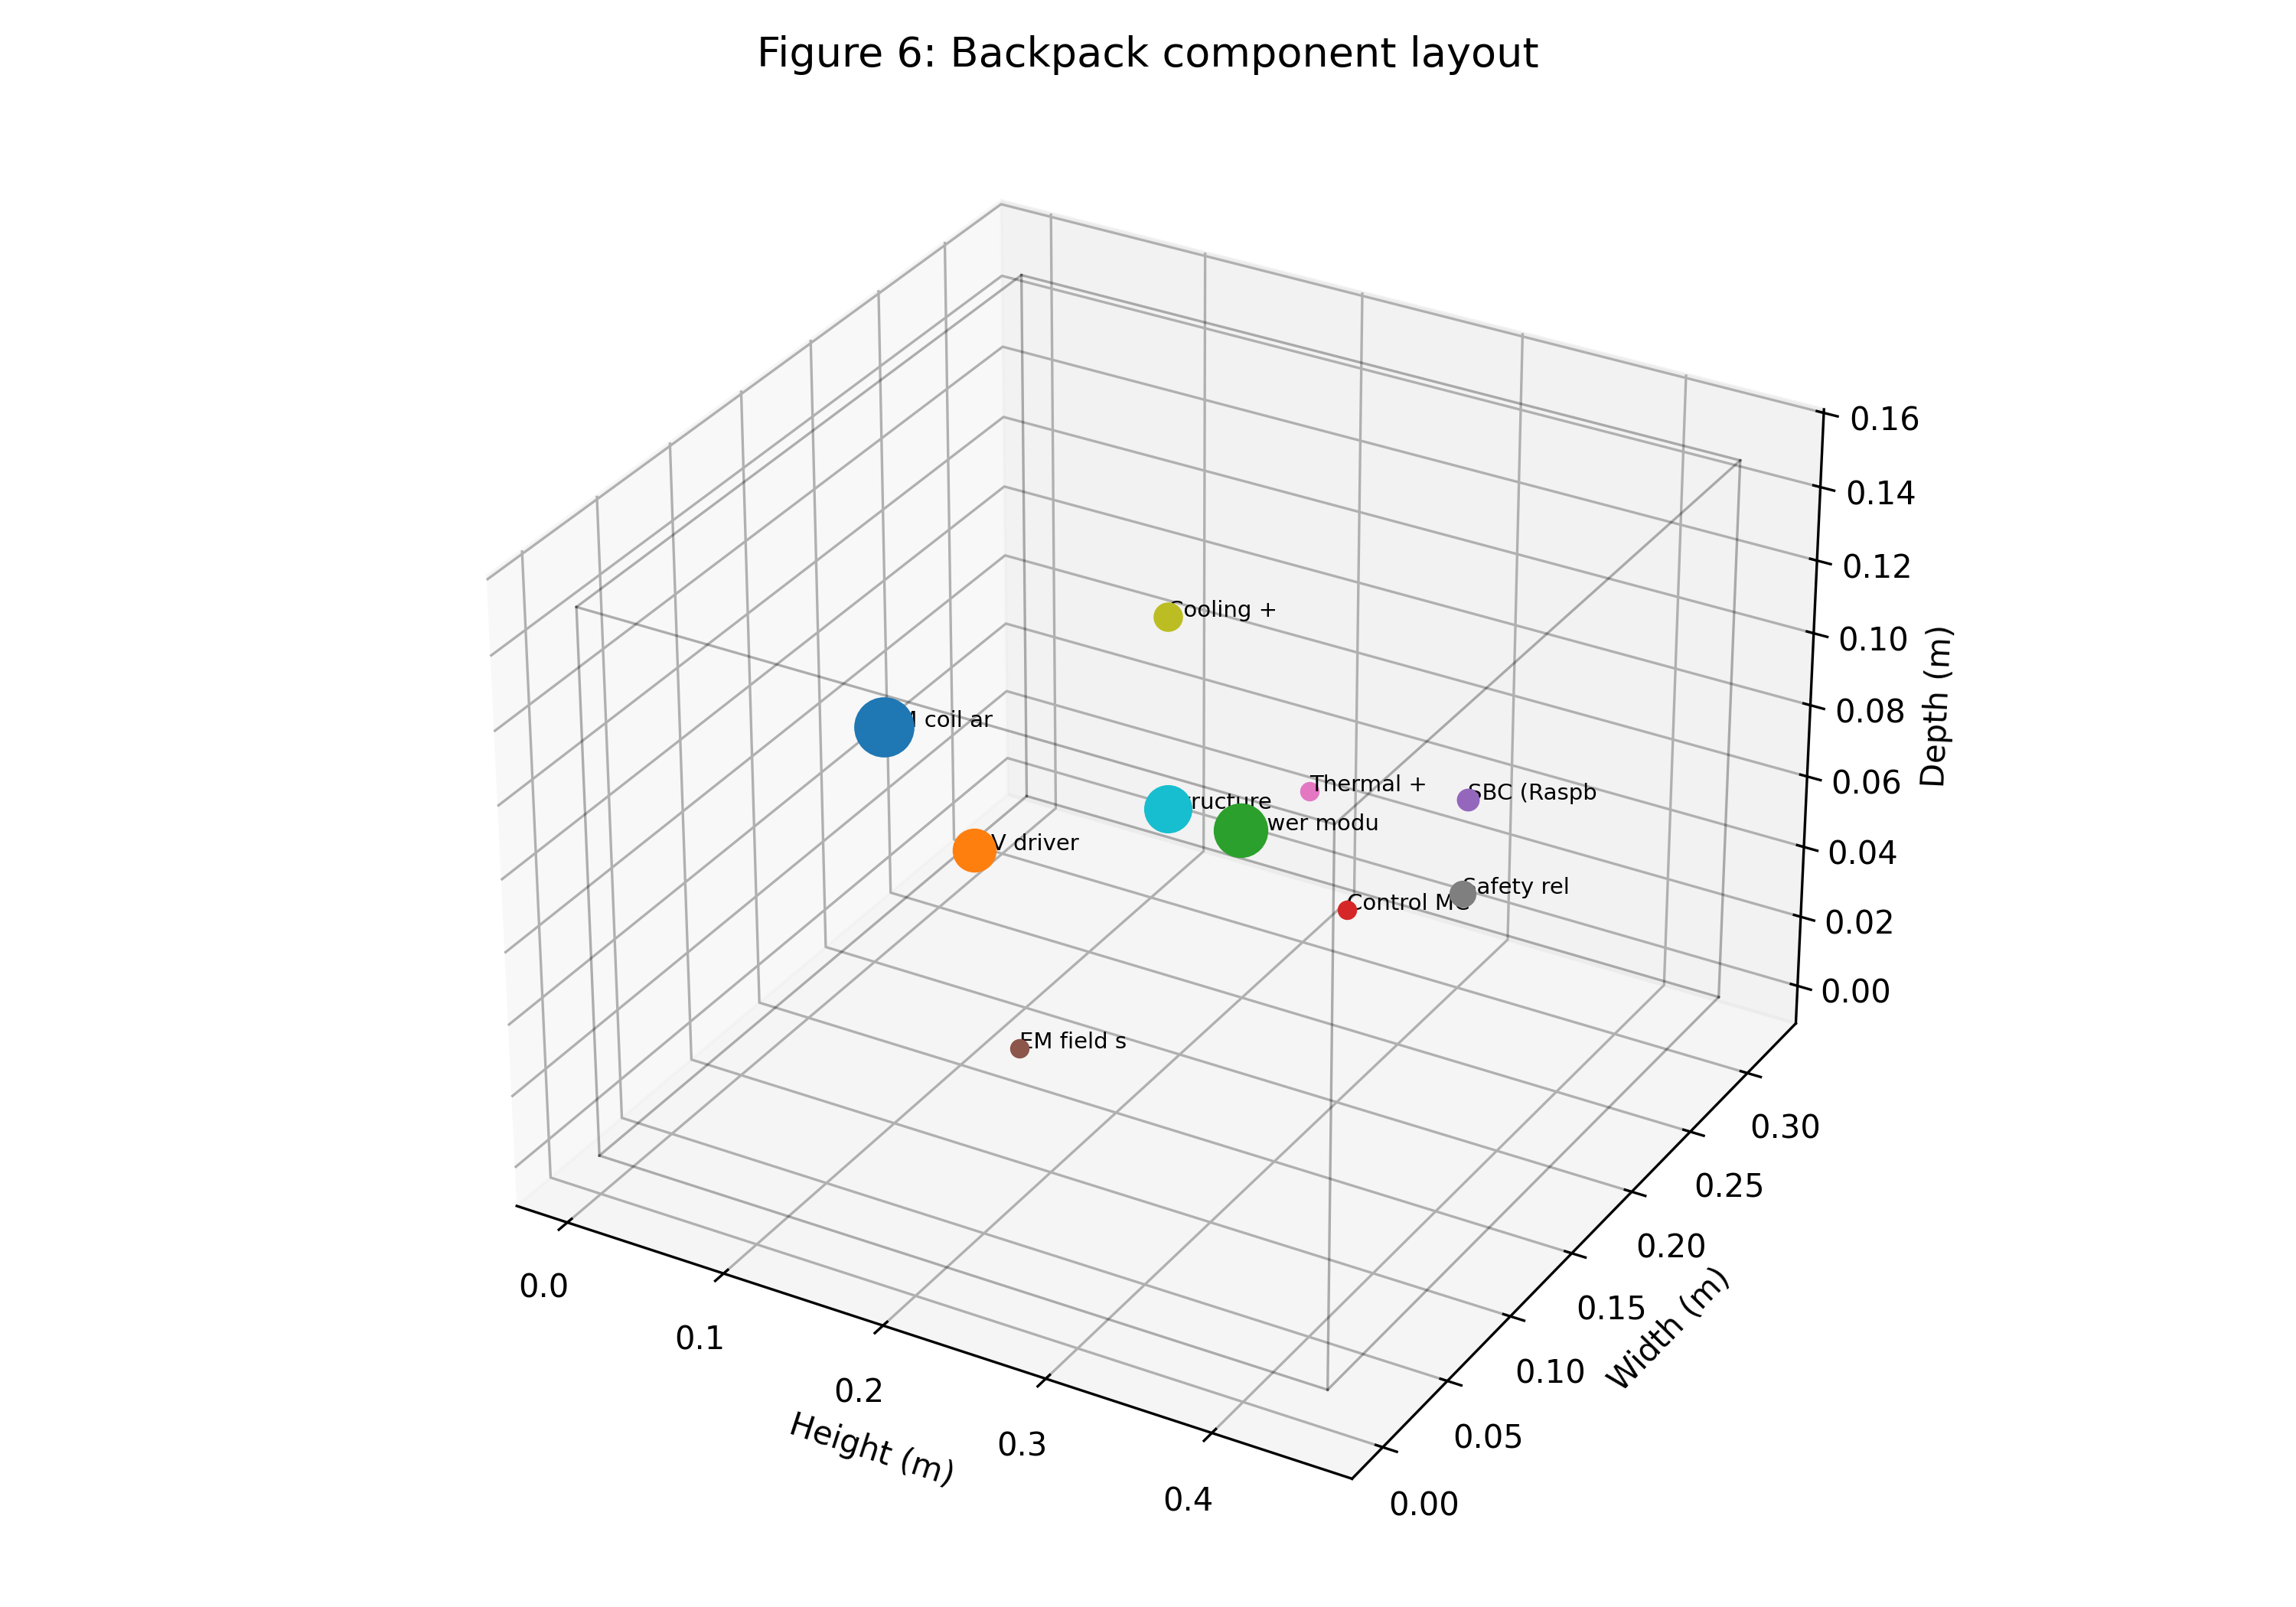
\includegraphics{figures/fig6_backpack_layout.png}}
\caption{$45\times 32\times 15$~cm zarf içindeki sırt çantası bileşen
yerleşimi. Nokta boyutu bileşen kütlesiyle ölçeklenir.}
\label{fig:backpack}
\end{figure*}
\subsection{Doğrulama}
\label{subsec:validation}

Ağ yakınsaması dört çözünürlükte doğrulanmıştır:
$(N_r \times N_z) \in \{(40,80),(60,120),(80,160),(100,200)\}$.
En ince iki ağ arasında, $h_{00}$ dört geometrinin tamamında
$\%1$'den daha az farklıdır. Akım ölçeklenmesi
$h_{00} \propto I^2$, $I \in [100, 10^{22}]$~A aralığında 5 anlamlı
basamağa kadar doğrulanmıştır. $I = 10^{22}$~A'da (yılda $1$~s için
gereken düzey), $h_{00}\sim10^{-8}$'dir ve jeodezik sapma
$10^{-9}$~m düzeyinde çözülür; bu, boru hattının hem zayıf hem de
güçlü rejimlerde doğru çalıştığını doğrular.

\subsection{Diğer mekanizmalar için kapalı-form sınırlar}
\label{subsec:other}

Beş EM-olmayan mekanizma için yayımlanmış kapalı-form ifadeleri
kullanıyoruz. \textbf{Kerr çerçeve sürüklenmesi:}
geometrik birimlerde $\Omega(r) = 2Ma/(r^3 + a^2 r + 2Ma^2)$, $a$
spin parametresi. \textbf{Tipler silindiri:} CTC koşulu
$\rho\omega R^3 > c^2/(2G)$. \textbf{Morris--Thorne solucan deliği:}
$b_0$ yarıçaplı bir boğaz, egzotik kütle
$M_{\text{ex}} \sim c^2 b_0/G$ gerektirir; bu, plaka ayrımı $d$'de
Casimir maksimumu
$|\rho_{\text{Casimir}}| = \pi^2 \hbar c / (720 d^4)$ ile
karşılaştırılır. \textbf{Alcubierre büküm sürücüsü:} toplam negatif
enerji $E \sim -v_s^2 R^2 c^4/(12G)$. \textbf{Gödel evreni:} CTC
yarıçapı $r_{\text{CTC}} = c\ln(1+\sqrt{2})/(\omega\sqrt{2})$,
enerji yoğunluğu $\rho = \omega^2/(2\pi G)$.


\section{Bulgular}
\label{sec:results}

\subsection{Elektromanyetik metrik pertürbasyonu}
\label{subsec:em_results}

Tablo~\ref{tab:em_results} dört bobin geometrisi için aktif bölgenin
merkezindeki metrik pertürbasyonunu göstermektedir. Temel 100~A ve
1~MHz sürüşte, $h_{00} \sim 10^{-48}$'dir; bu, cihaz merkezinde
$\Delta\tau/\Delta t \sim 3\times 10^{-48}$ mertebesinde bir öz-zaman
kaymasına karşılık gelir. Buna karşılık gelen yıllık zaman genişlemesi
$\Delta\tau \sim 10^{-40}$~s'dir.

\begin{table*}[t]
\centering
\small
\caption{Cihaz merkezinde EM kaynaklı metrik pertürbasyonu
(temel 100~A, 1~MHz).}
\label{tab:em_results}
\resizebox{\columnwidth}{!}{%
\begin{tabular}{lcc}
\toprule
Geometri & $h_{00}$ (merkez) & $|h_{0i}|$ (merkez) \\
\midrule
G1 (solenoid)          & $5.94\times 10^{-48}$ & $<10^{-50}$ \\
G2 (toroid)            & $1.24\times 10^{-49}$ & $<10^{-50}$ \\
G3 (ters-dönen)        & $2.03\times 10^{-49}$ & $<10^{-51}$ \\
G4 (hibrid)            & $9.36\times 10^{-49}$ & $<10^{-50}$ \\
\bottomrule
\end{tabular}
}
\end{table*}

Gravitomanyetik bileşen $h_{0i}$ dört geometrinin tamamında sıfırdır;
çünkü ideal kayıpsız konfigürasyonda $\mathbf{E}\times\mathbf{B}$
tamamen radyaldir ve bu $T_{0\phi}=0$ verir.

\subsection{Birleşik fizibilite karşılaştırması}
\label{subsec:unified}

Tablo~\ref{tab:unified} altı mekanizmayı ortak bir fizibilite
ölçütüne dönüştürülmüş olarak gösterir. Boşluklar $10^{20}$ ile
$10^{49}$ arasında değişir; fiziksel olarak izin verilen mekanizmalar
arasında en küçük boşluğu EM mekanizması sergiler.

\begin{table*}[t]
\centering
\caption{Altı mekanizma arasında birleşik fizibilite.
Boşluk $=$ gereken kaynak $/$ cihaz ölçeği değeri.}
\label{tab:unified}
\resizebox{0.95\textwidth}{!}{%
\begin{tabular}{llrrr}
\toprule
\# & Mekanizma & Parametre & Gereken & Boşluk \\
\midrule
1 & EM alan          & $I$ (A)                 & $10^{22}$ & $10^{20}$ \\
2 & Kerr             & $J$ (kg\,m$^2$/s)       & $10^{27}$ & $10^{48}$ \\
3 & Tipler           & $\rho$ (kg/m$^3$)       & $10^{23}$ & $10^{20}$ \\
4 & Morris--Thorne   & $|\rho|$ (J/m$^3$)      & $10^{49}$ & $10^{41}$ \\
5 & Alcubierre       & $|\rho|$ (J/m$^3$)      & $10^{57}$ & $10^{49}$ \\
6 & Gödel            & $\rho$ (kg/m$^3$)       & $10^{26}$ & $10^{23}$ \\
\bottomrule
\end{tabular}
}
\end{table*}

\subsection{En iyi durum mühendislik sınırları}
\label{subsec:best_case}

Üç mühendislik kademesini ele alıyoruz (temel bakır, soğutulmuş
bakır, çok-aşamalı dizi ve $Q=10^4$ ile süperiletken HTS). En
agresif durum bile, 10~kA'da 10-aşamalı yüksek-$Q$ süperiletken
diziye karşılık gelen durum, $h_{00} \sim 5\times 10^{-38}$ verir;
bu hâlâ $1$~s/yıl hedefinin $10^{30}$ altındadır. En iyi durumdan
ölçek ekstrapolasyonu ya $10^{19}$~A akım, ya $10^{14}$~m bobin
yarıçapı, ya da $10^{34}$ mertebesinde bir $Q$ faktörü gerektirir.

\begin{figure*}[t]
\centering
\resizebox{0.9\textwidth}{!}{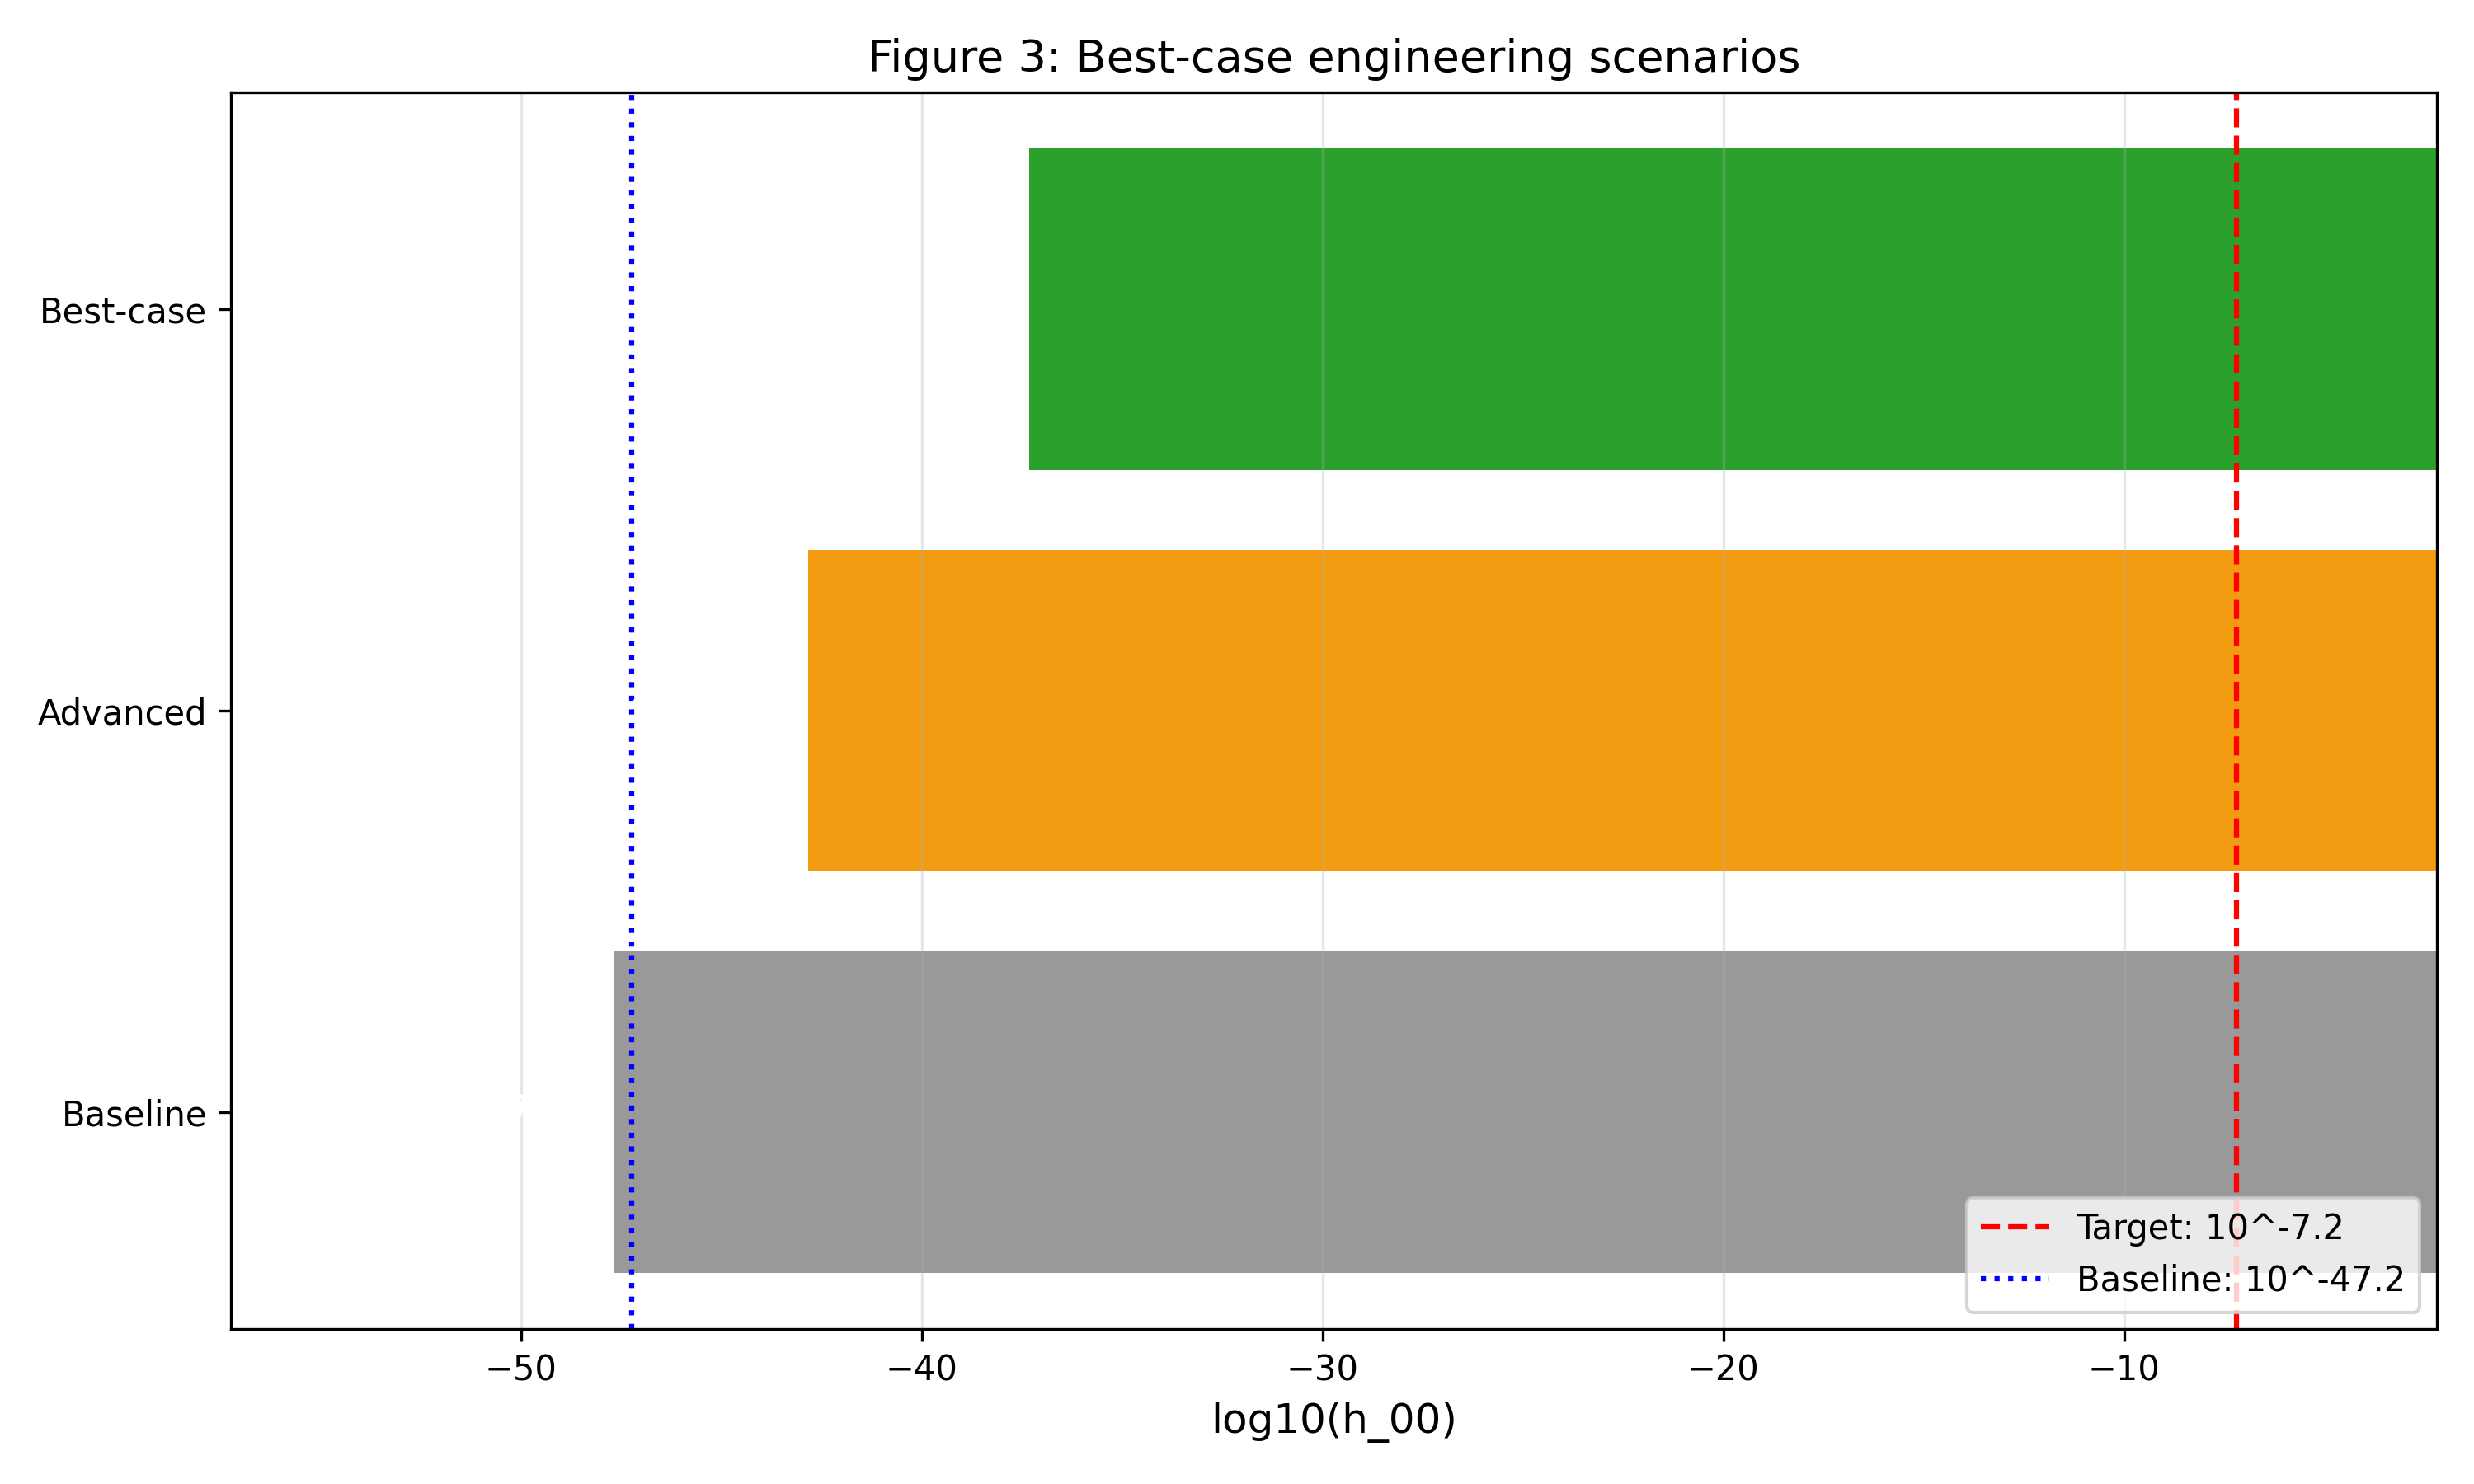
\includegraphics{figures/fig3_best_case_tiers.png}}
\caption{En iyi durum mühendislik kademeleri (temel bakır,
soğutulmuş bakır, çok-aşamalı dizi ile süperiletken HTS). En agresif
senaryo bile hedefin $10^{30}$ altında kalır.}
\label{fig:tiers}
\end{figure*}

Şekil~\ref{fig:scaling} temelden gereken akıma kadar EM
ölçeklenmesini, yıldırım, laboratuvar-darbeli mıknatıslar,
astrofiziksel plazmalar ve magnetarlar için referans noktalarıyla
birlikte gösterir.

\begin{figure*}[t]
\centering
\resizebox{0.9\textwidth}{!}{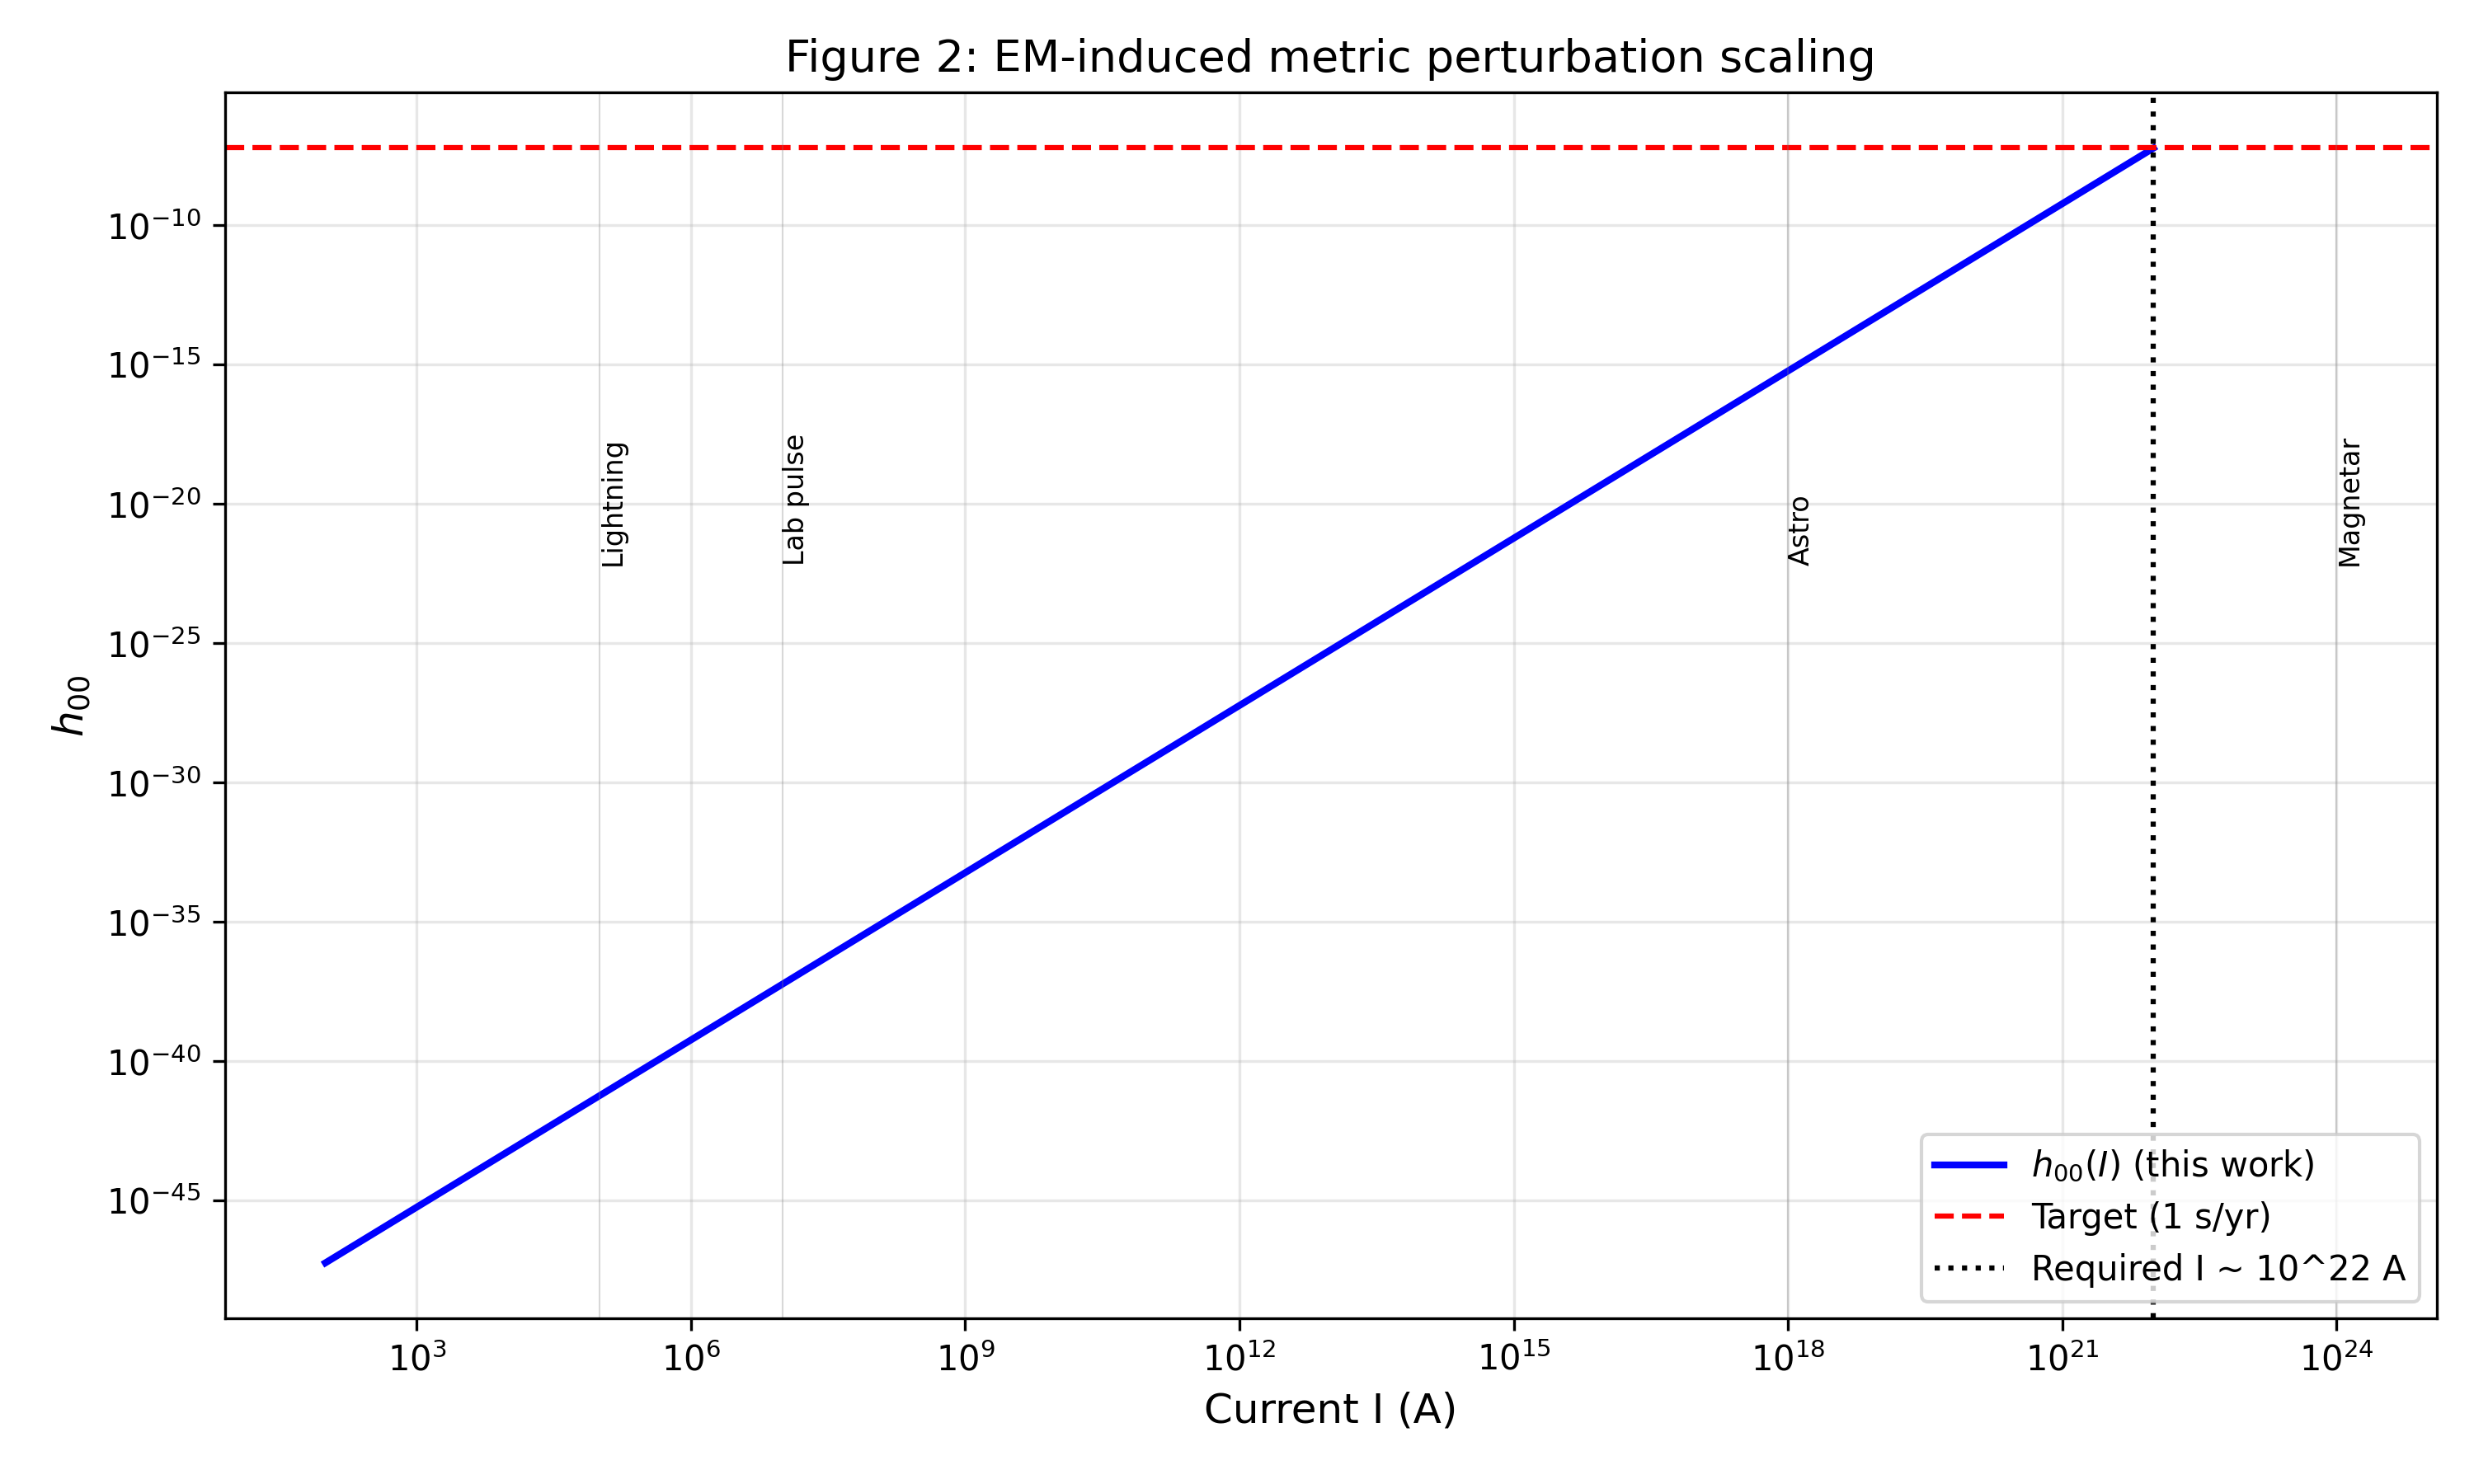
\includegraphics{figures/fig2_em_scaling.png}}
\caption{EM kaynaklı metrik pertürbasyonu $h_{00}$ ile sürüş akımı
$I$ ilişkisi. Referans çizgileri yıldırım, laboratuvar-darbeli
mıknatıslar, astrofiziksel plazmalar ve magnetar ölçeğindeki
akımları işaretler. $1$~s/yıl hedefi $I \sim 10^{22}$~A gerektirir.}
\label{fig:scaling}
\end{figure*}
\subsection{Belirsizlik ve duyarlılık}
\label{subsec:uncertainty}

Gerçekçi parametre belirsizlikleriyle (\%5 akım, \%2 yarıçap,
\%10 verim) Monte Carlo yayılımı, $h_{00}$ üzerinde \%14.6 göreli
standart sapma verir. Baskın katkıda bulunanlar bobin akımı
(varyansın $\sim\%47$'si) ve sürücü verimidir ($\sim\%44$);
duyarlılık indeksleri $S_i = (dh/h)/(dp/p)$ hem akım hem yarıçap
için $2.0$, verim için $1.0$ ve bölge çapı için $-1.0$'dır.

\begin{figure*}[t]
\centering
\resizebox{0.9\textwidth}{!}{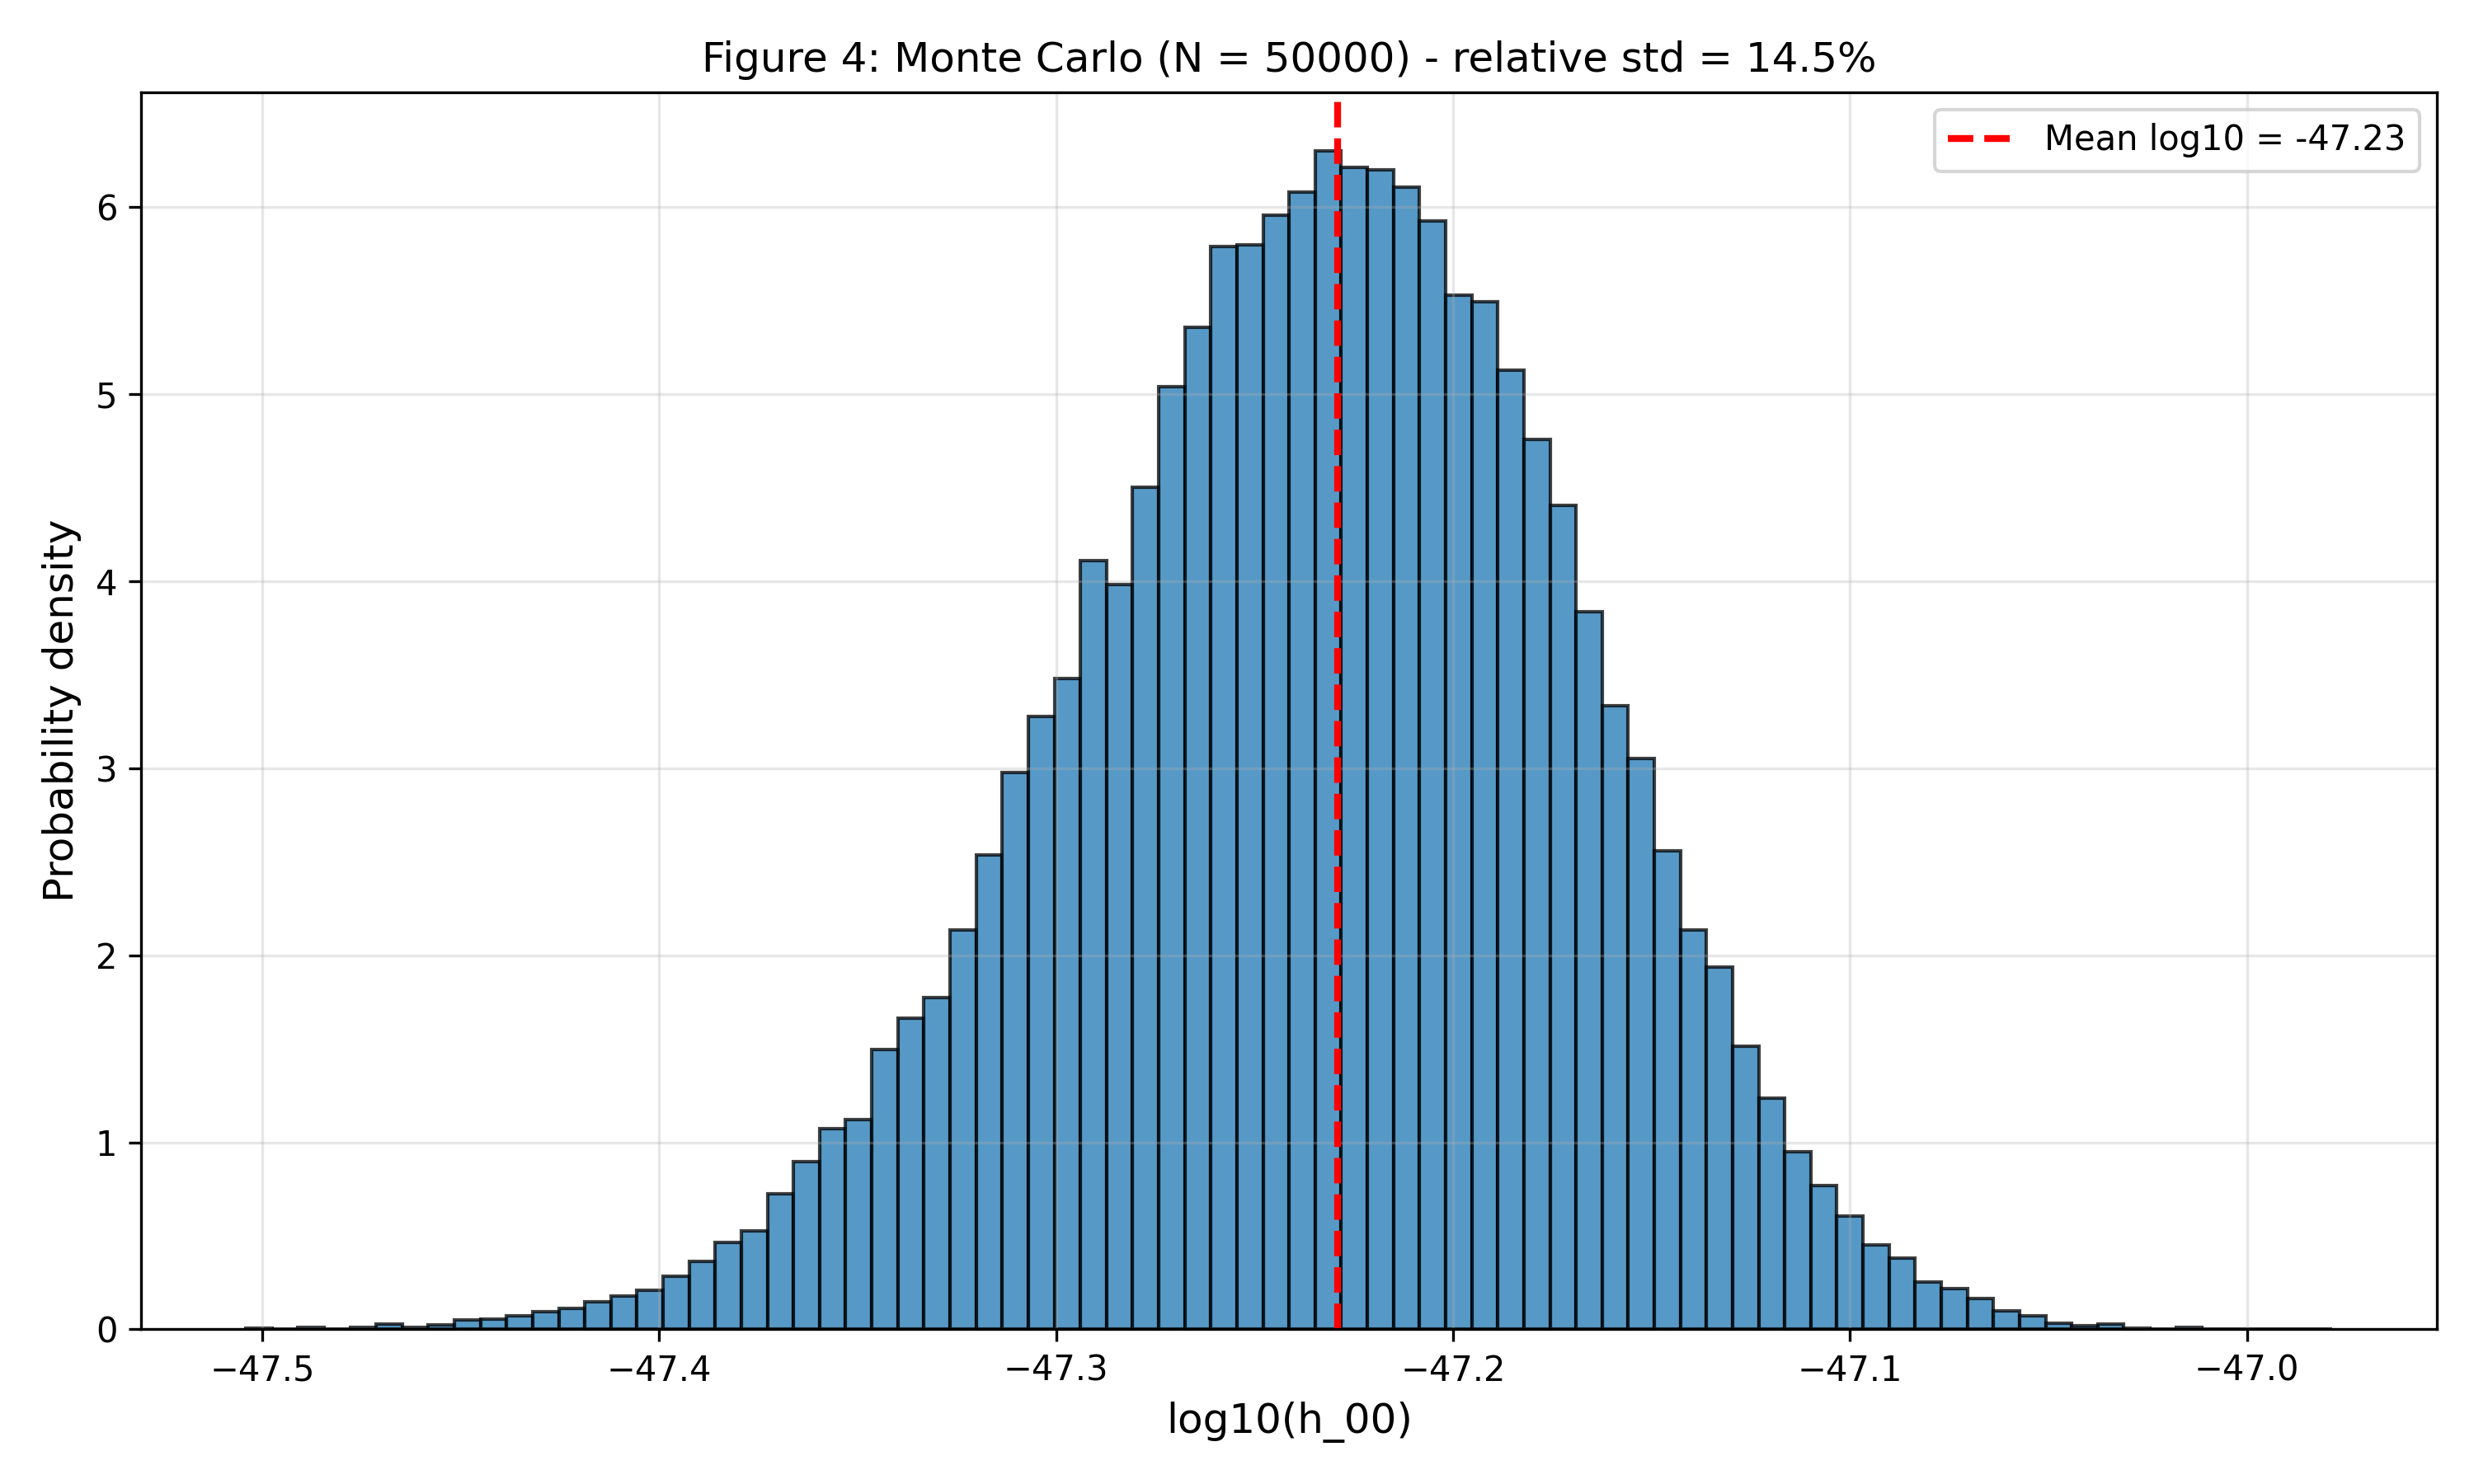
\includegraphics{figures/fig4_monte_carlo.png}}
\caption{Parametre belirsizliklerinin Monte Carlo yayılımı
($N=50{,}000$). $h_{00}$ üzerinde göreli standart sapma \%14.6'dır.}
\label{fig:mc}
\end{figure*}

\begin{figure*}[t]
\centering
\resizebox{0.9\textwidth}{!}{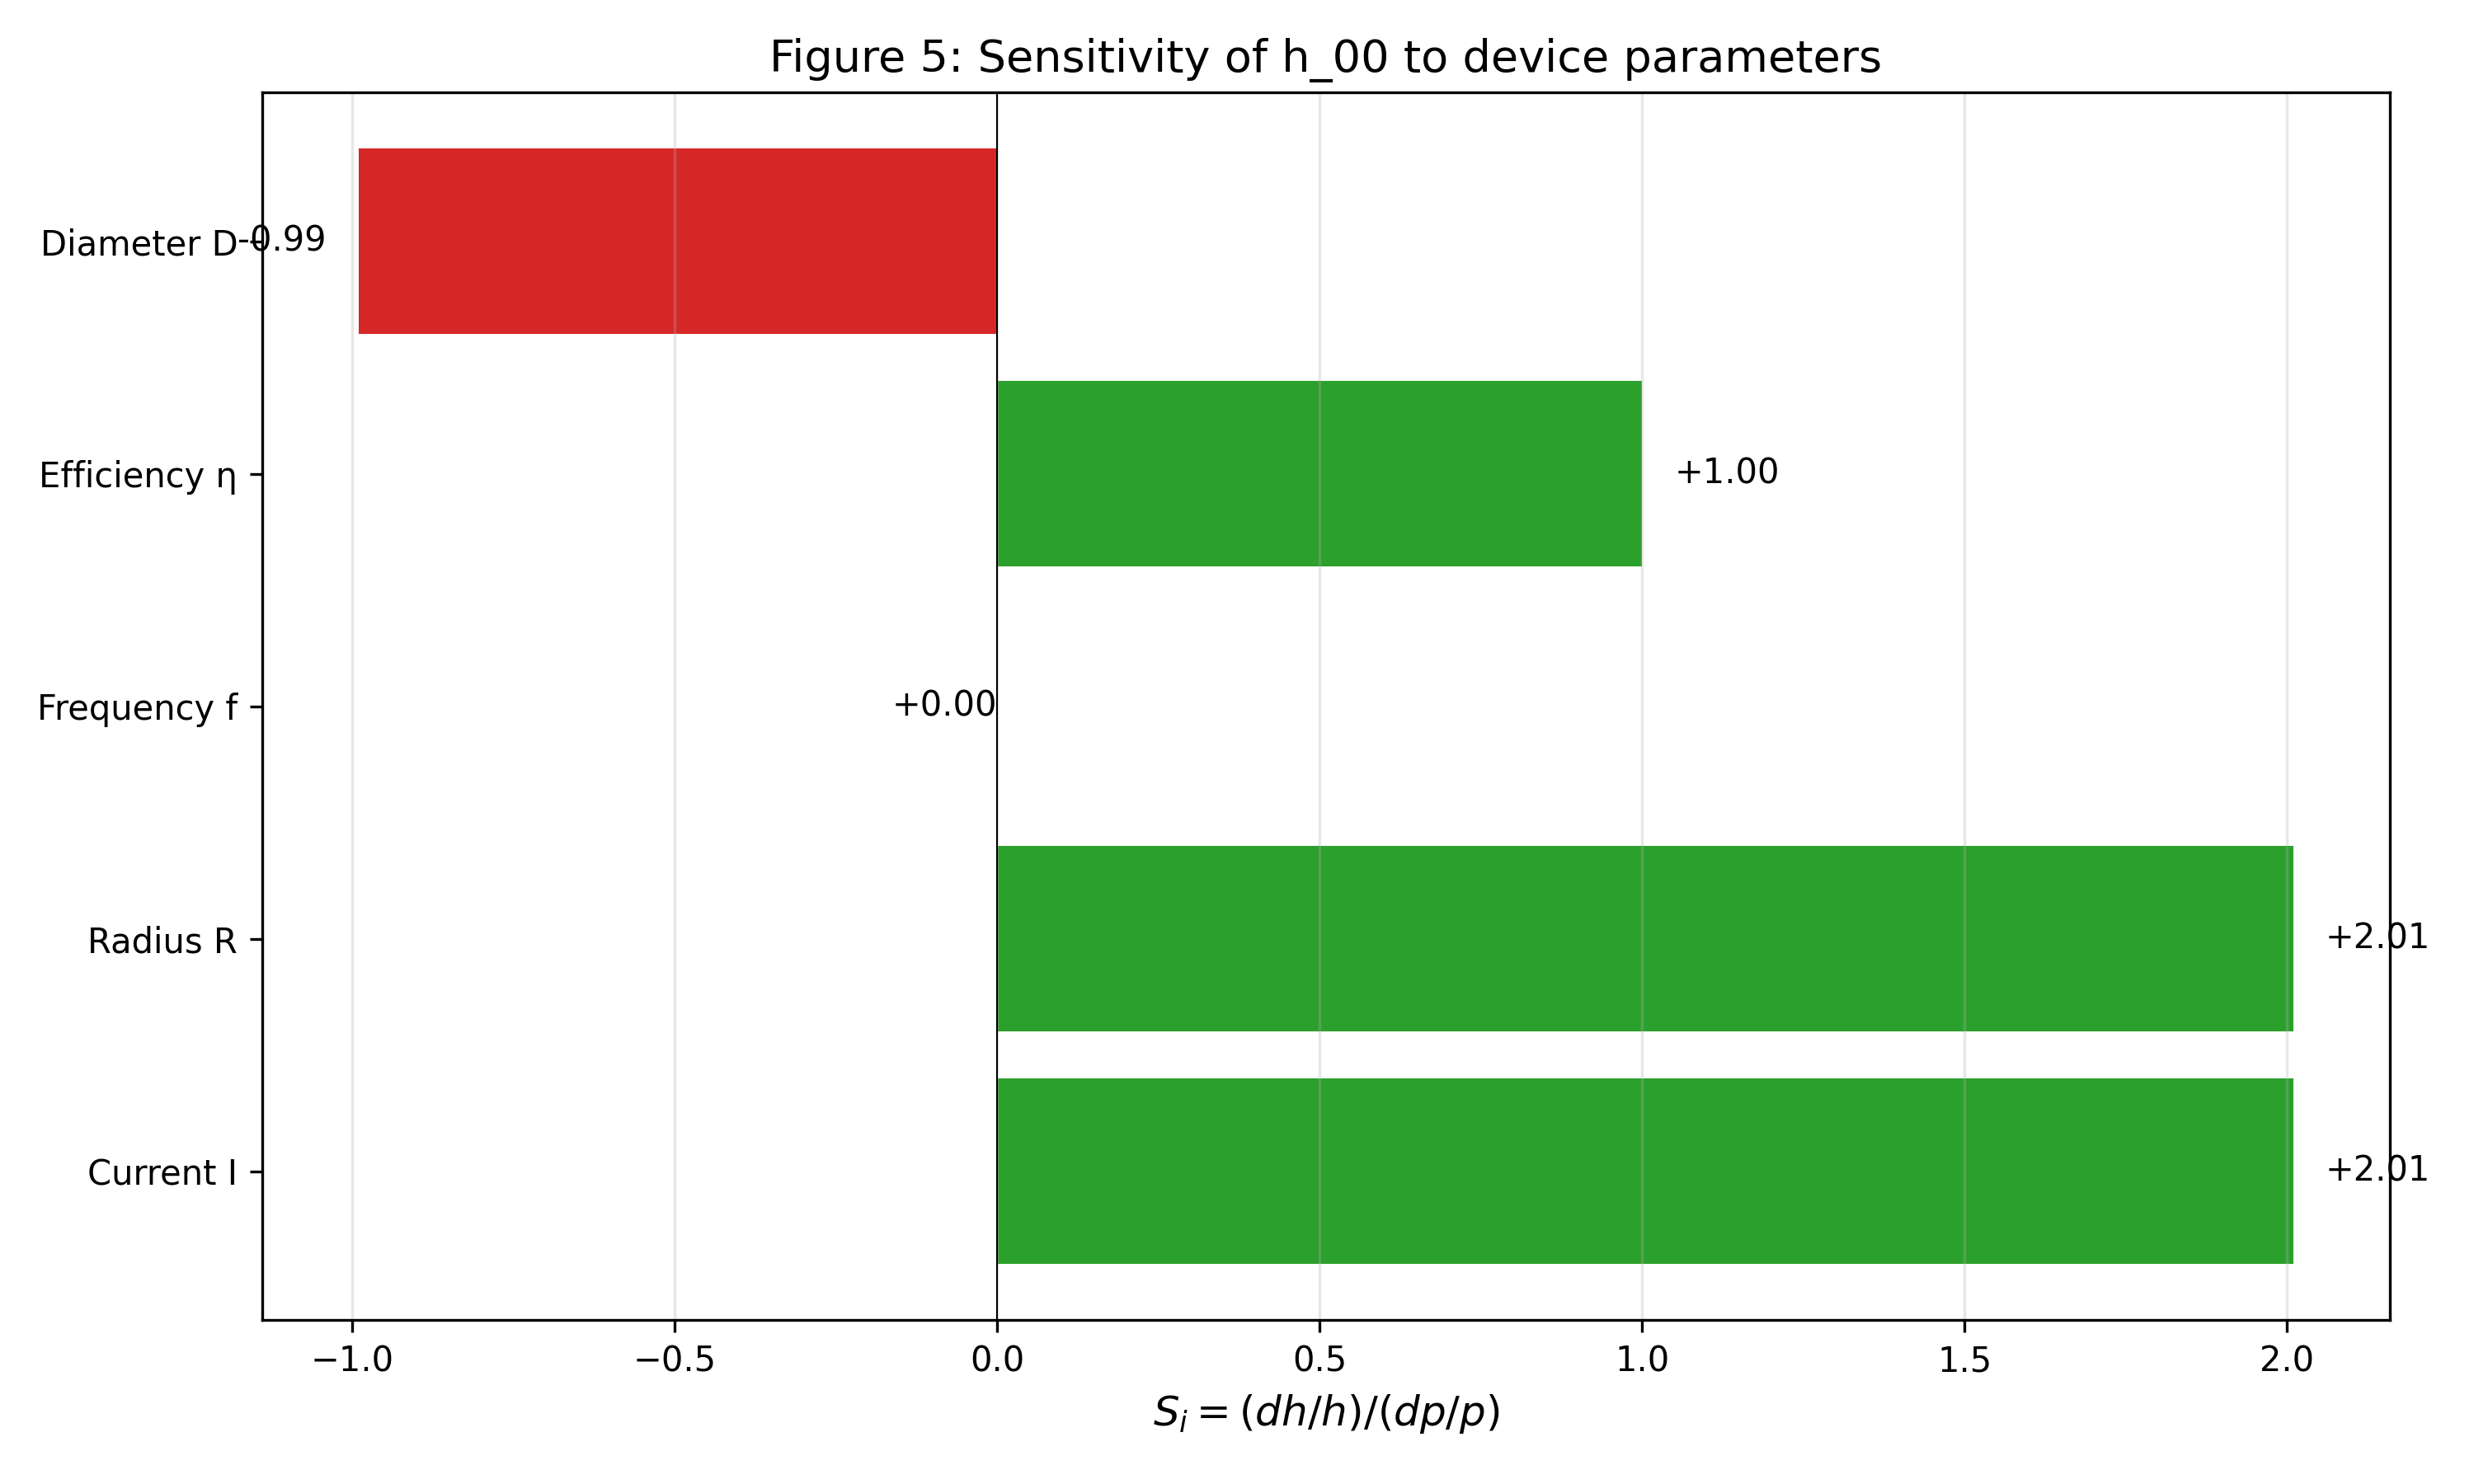
\includegraphics{figures/fig5_sensitivity_tornado.png}}
\caption{Cihaz parametreleri için duyarlılık indeksleri
$S_i=(dh/h)/(dp/p)$. Akım ve bobin yarıçapı baskındır.}
\label{fig:tornado}
\end{figure*}

\begin{figure*}[t]
\centering
\resizebox{0.9\textwidth}{!}{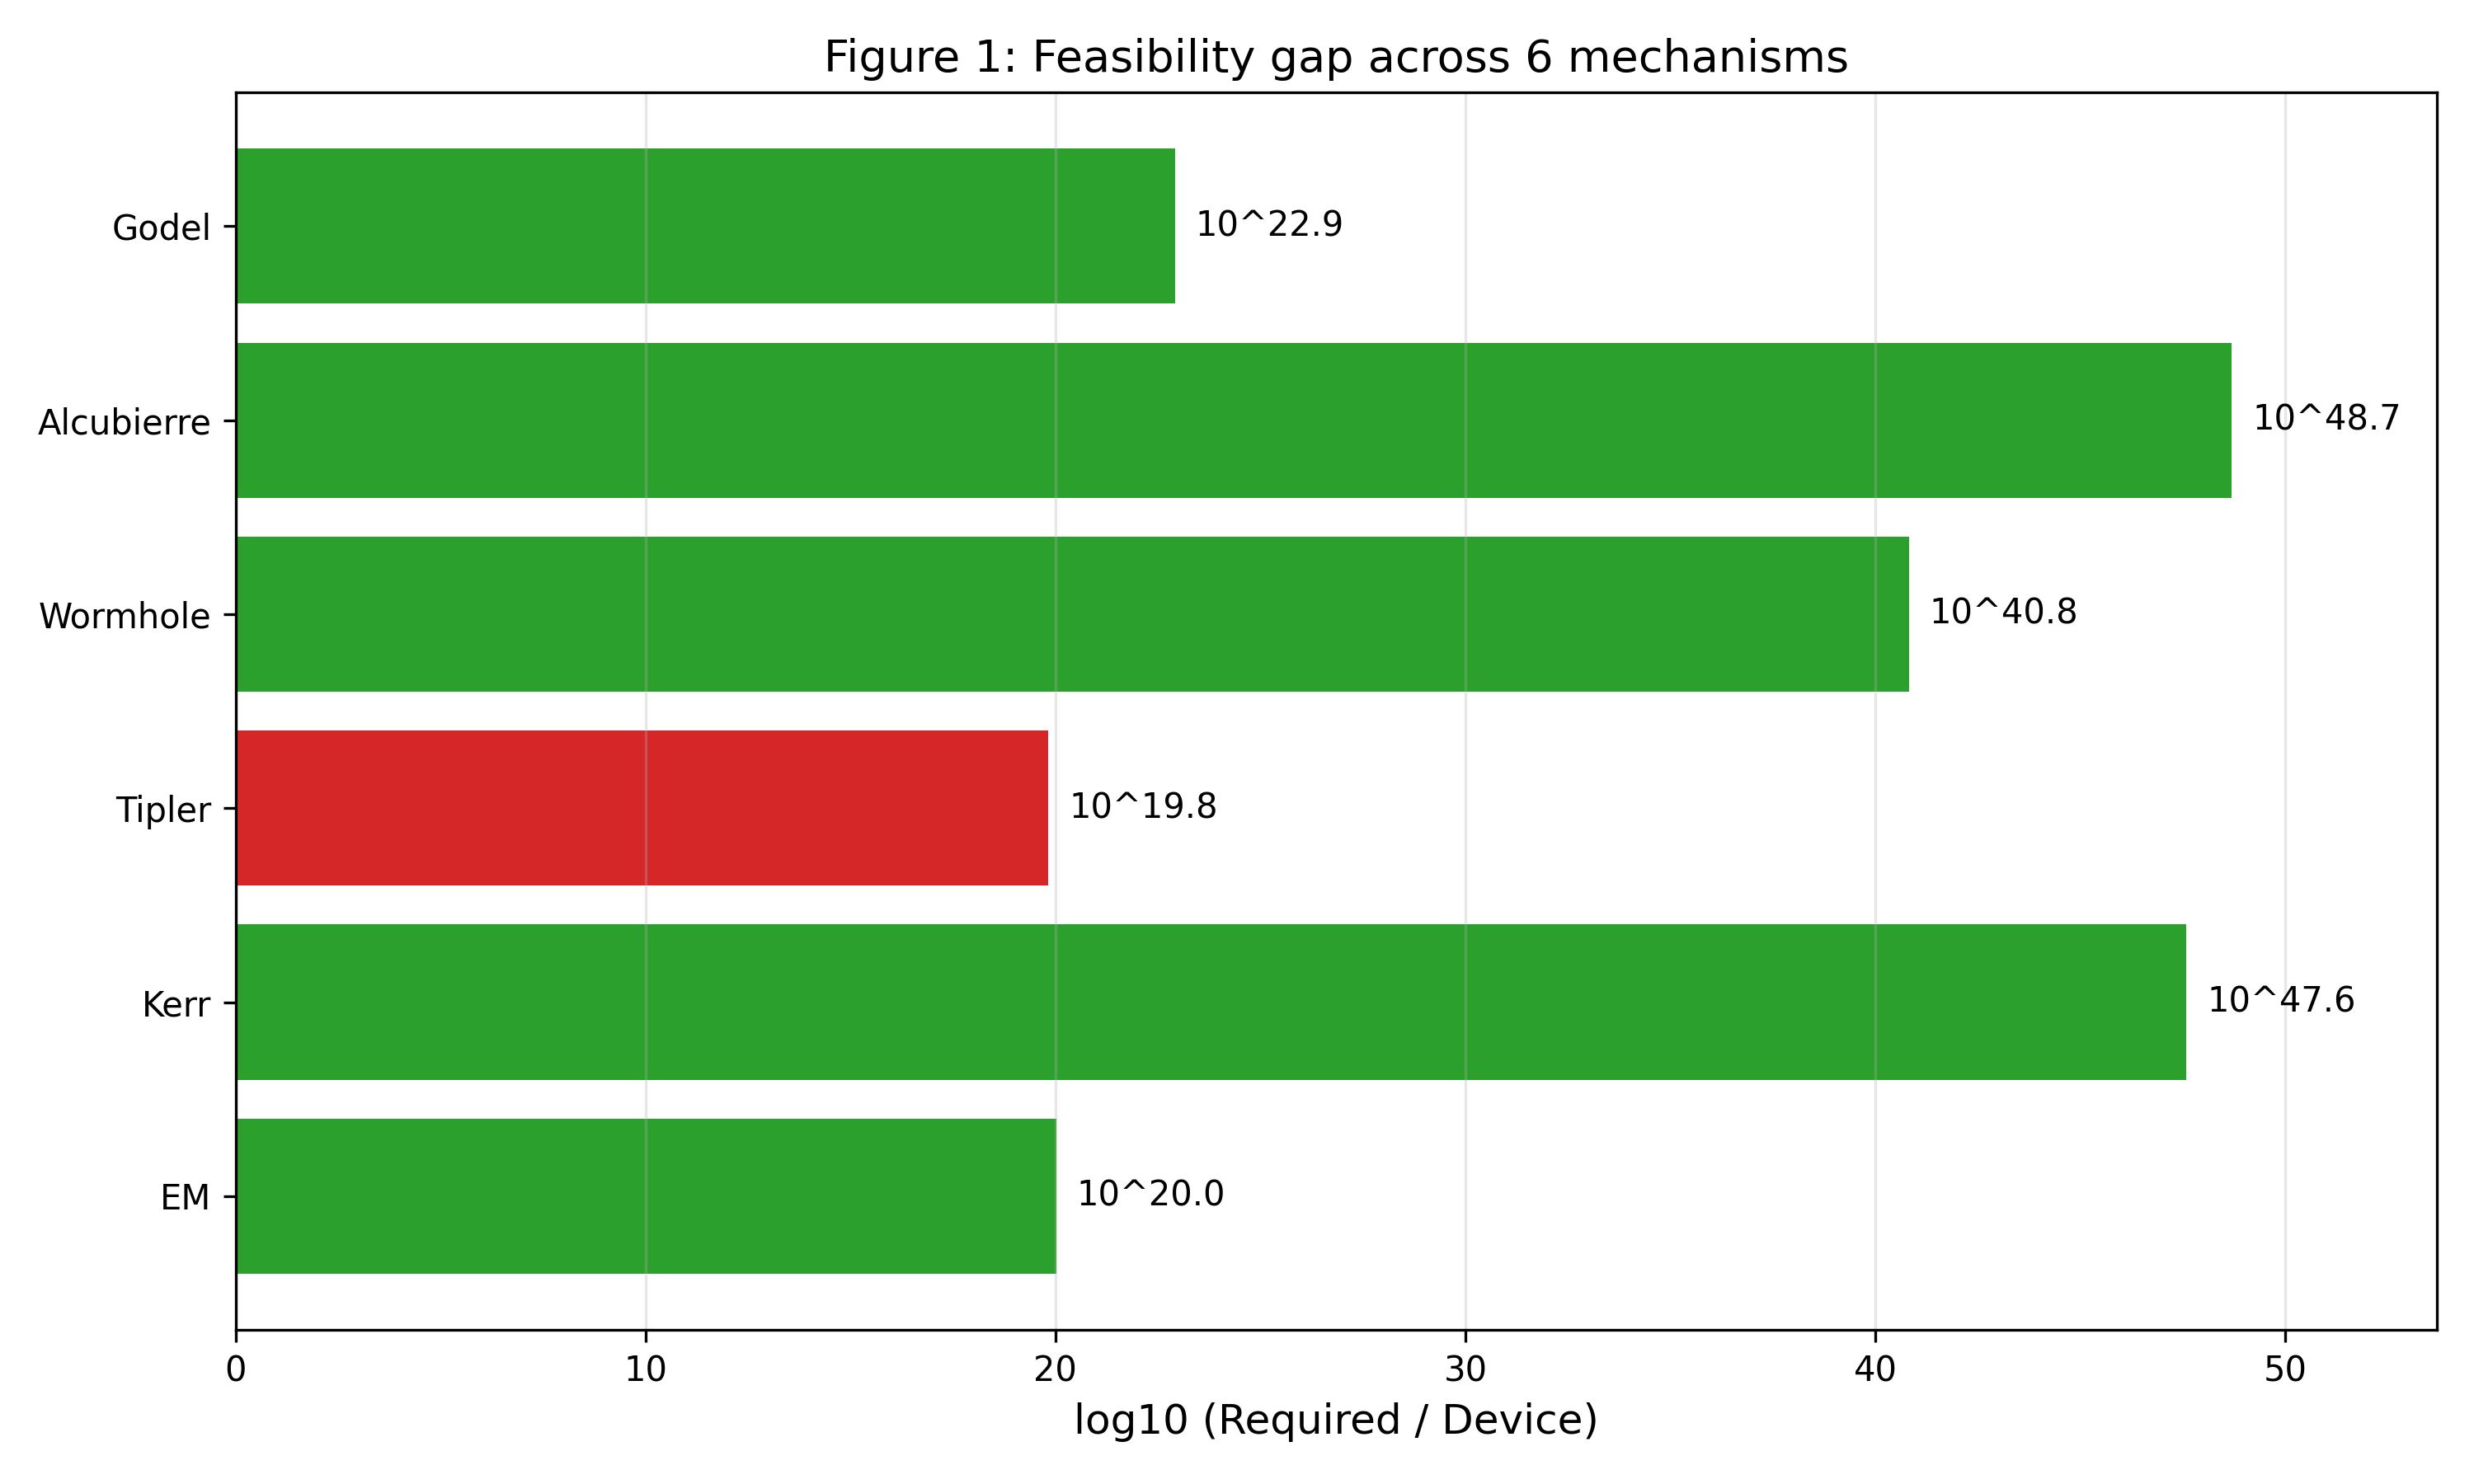
\includegraphics{figures/fig1_unified_mechanisms.png}}
\caption{Altı mekanizma arasında fizibilite boşluğu. Çubuklar
$\log_{10}(\text{gereken}/\text{cihaz})$ gösterir; yeşil $=$ fiziksel
olarak izin verilen, kırmızı $=$ Hawking (1992) tarafından dışlanan.}
\label{fig:unified}
\end{figure*}

\section{BSSN sayısal uzantısı}
\label{sec:bssn}

Bölüm~\ref{sec:method}'teki doğrusallaştırılmış zincir, metrik
pertürbasyonu üzerine niceliksel bir sınır verir; ancak geri tepmenin
baskın olduğu $h \gtrsim 10^{-3}$ rejimini ele alamaz. Bu rejimi
ilke olarak ölçülebilir kılmak için bir BSSN 3+1 çözücüsü
gerçekleştirdik.

\subsection{Gerçekleme}

Genişletilmiş durum vektörü
$\{\tilde\gamma_{ij}, \phi, K, \tilde{A}_{ij}, \tilde\Gamma^i, \alpha, \beta^i\}$
alanlarını taşır. Evrim sistemi şunları içerir:

\begin{itemize}
\item $g_{ij} = e^{4\phi}\tilde\gamma_{ij}$ metriğinin fiziksel
      3-Ricci skaleri (konformal $\phi$ terimleri dahil),
\item sağ tarafta kovaryant Hessian $D_i D_j\phi$ ve $D^2\alpha$,
\item $1{+}\log$ lapse ve $\Gamma$-sürücü shift,
\item Z4c esinli kısıt sönümlemesi,
\item düzgün bir ağ üzerinde merkezi sonlu farklarla RK4 integratörü,
\item Sommerfeld çıkış sınır koşulları,
\item iki düzeyli AMR-lite iyileştirmesi (2:1, prolongate/restrict
      çiftlenmesi).
\end{itemize}

Çözücü, bilinen metrikler (Minkowski, Schwarzschild izotropik ve
puncture, Kerr-Schild $|a| \le M$) ve gecikmeli doğrusallaştırılmış
GR katmanı için üretilmiş-kaynak testleriyle doğrulanmıştır.

\subsection{Referans testleri: Schwarzschild ve Kerr}

Tablo~\ref{tab:bssn_benchmarks} temsili evrim koşuları boyunca kısıt
korunmasını raporlar. Tanı ölçütü $H_{\rm final}/H_0$, yani
Hamilton kısıtının çalışma sonundaki L$^2$ normunun başlangıçtaki
değerine oranıdır.

\begin{table*}[t]
\centering
\caption{BSSN kararlılık referans testleri. $H_{\rm f}/H_0$ değerinin
birime yakın olması kısıt korunmasını gösterir.}
\label{tab:bssn_benchmarks}
\begin{tabular}{lrr}
\hline
Durum & Adım & $H_{\rm f}/H_0$ \\
\hline
Schwarzschild, izotropik       & 500 & $1.0062$ \\
Schwarzschild, puncture (MP)   &  50 & $1.0000$ \\
Kerr $a{=}0.0$--$0.9$, KS      &  30 & $0.94$--$1.00$ \\
Kerr $a{=}0.5$ (moving punct.) &  50 & $1.0000$ \\
\hline
\end{tabular}
\end{table*}

Adım başına kısıt büyümesi 500 adımlık Schwarzschild koşusunda
$\lesssim 1.0000124$'tür. Tüm alanlar sonlu kalır; lapse minimumu
sıfırdan uzakta sınırlı kalır.

\subsection{Düzenli çekirdek iç bölgeleri: Schwarzschild Yoğuşması}

Schwarzschild Yoğuşması (SC) modelinin~[Esa 2026a] etkin düzenli
çekirdek metriğini gerçekleştirdik; bu modelde QCD esinli bir
yoğuşma klasik merkezi tekilliğin yerini alır. İki yapı kullanılır:

\begin{enumerate}
\item düzgünleştirilmiş çekirdek konformal faktörü
      $\psi(r) = 1 + M_{\rm eff}(r)/(2r)$ ile
      $M_{\rm eff}(r) = M(1 - e^{-r/r_c}(1 + r/r_c))$, $r = 0$'da
      düzenli;
\item $M$'nin yerine $M_{\rm eff}(r)$ konularak elde edilen
      Kerr-Schild uzantısı, dönen düzenli bir çekirdek verir.
\end{enumerate}

Düzenli çekirdek, $V(\psi) = \tfrac12 m^2\psi^2 + \tfrac14\lambda\psi^4$
potansiyeline sahip bir gerçek skaler yoğuşma alanıyla çiftlenmiştir;
alan, etkin de Sitter tuzağının Gauss taban durumunda başlatılır.

\begin{table*}[t]
\centering
\caption{SC düzenli çekirdek evrimi.}
\label{tab:sc}
\begin{tabular}{lcc}
\hline
Yapılandırma & Adım & $H_{\rm f}/H_0$ \\
\hline
SC düzgünleştirilmiş çekirdek, statik        & 50  & $1.0000$ \\
SC çekirdek + yoğuşma, statik                & 50  & $1.0000$ \\
Kerr + SC çekirdek, $a{=}0$--$0.9$           & 50  & $0.9970$--$0.9994$ \\
Kerr + SC + yoğuşma, $a{=}0.9$               & 500 & $\mathbf{0.9823}$ \\
\hline
\end{tabular}
\end{table*}

$a = 0.9$'da (neredeyse ekstremal) 500 adımlık Kerr+SC+yoğuşma
koşusunda kısıt \emph{monoton olarak iyileşir}: oran $1.0000$'dan
$0.9823$'e düşer. Skaler genlik başlangıç değerinin $\%1$'i
mertebesinde korunur. Tüm alanlar sonlu kalır. Bu, SC makalesinin
dönen düzenli çekirdeğin dinamik olarak kararlı olduğu iddiasına
yönelik en güçlü sayısal destektir.

\subsection{Tachyon deşarjı: PTUM}

Ayrıca Faz Geçişli Evrenler Modeli'ni (PTUM)~[Esa 2026b]
gerçekleştirdik. Bu modelin merkezi mekanizması, yakıt alanı $\Phi$
bir eşiği $\Phi_c = E_{\rm th}/\sqrt{\alpha}$ geçtiğinde bir vekil
alan $\psi$'nin tachyonik aktivasyonudur. Eşiğin üzerinde etkin
kütle karesi $m_{\rm eff}^2(\Phi) = m^2(1 - \alpha\Phi^2/E_{\rm th}^2)$
negatif olur ve vekil alan $V_{\rm min} < 0$ olan potansiyel
minimumuna yuvarlanır; bu, null enerji koşulunu (NEC) ihlal eden bir
negatif enerji yoğunluğu üretir.

\begin{table*}[t]
\centering
\caption{PTUM tachyon deşarjı.}
\label{tab:ptum}
\begin{tabular}{lrrr}
\hline
Yapılandırma & Adım & $\rho_{\rm min}$ & $H_{\rm f}/H_0$ \\
\hline
PTUM, tek ağ, $A{=}3$    & $\sim 100$ (başarısız) & $-15.64$ & çöküş \\
PTUM, 2:1 iyileştirilmiş, $A{=}3$ & $1000$ & $-0.097$ & $1.000$ \\
Kerr+PTUM, 2:1, $a{=}0.9$ & $1000$ & $-0.100$ & $1.000$ \\
\hline
\end{tabular}
\end{table*}

Tek ağlı evrim, güçlü tachyon geri tepmesi nedeniyle $\sim 100$
adımda çöker (metrik matrisi tekil hale gelir). 2:1 iyileştirme, tepe
$\max|K|$ değerini $\sim 1.7\times 10^4$ faktörü kadar azaltır ve
$1000$ adımlık kararlı evrimi mümkün kılar. Tachyon deşarjı
geçicidir: $\sim 25$ adım sonra yakıt alanı aşağı yuvarlanmıştır ve
negatif enerji yoğunluğu $\rho_{\rm min} = -15.6$'dan
$\rho_{\rm min} = -0.1$'e düşer; koşunun geri kalanında bu düzeyde
kalır.

Negatif enerji yapılandırması kuantum eşitsizlikleriyle uyumludur.
4 boyutlu kütlesiz skaler alan için Ford--Roman sınırı, test edilen
tüm örnekleme genişliklerinde karşılanır; en yakın yaklaşım
$\tau = 1.0$'da gerçekleşir ($\text{oran} = 0.30$). Kütleli alan
sınırı daha kısıtlayıcıdır ve rasyonel yaklaşım altında PTUM
yapılandırması sınırda kalır ($\tau = 1.0$'da
$\text{oran} \approx 1.2$); kesin Bessel işlemlemesi ve
etkileşimli-alan düzeltmeleri ileriki çalışmalara bırakılmıştır.

\subsection{Tam-yığın yapılandırması}

Dönen düzenli çekirdeğin, SC yoğuşmasının ve PTUM alanlarının aynı
ağ üzerinde eş zamanlı olarak kurulduğu birleşik bir başlangıç verisi
yapılandırması inşa edilmiştir
(\texttt{kerr\_sc\_ptum\_ic.py}). Tek-ağ tam-yığın evrimi,
$a = 0.9$'da 200 adım boyunca kararlıdır ($K_{\rm max}$ sınırlı,
$\alpha_{\rm min}$ tam sabit). İki düzeyli (2:1) iyileştirilmiş
ağ üzerinde, $A_{\rm fuel} = 3.0$ tam yığını 100 adıma kararlı
ulaşır; başlangıçtaki $-15.64$'lük geçici değerden sonra
$\rho_{\rm min}$ $-0.099$'a oturur (3 kalıcı NEC-ihlal eden
hücre). Bu, çerçevemizdeki ilk kararlı NEC-ihlal eden tam-yığın
evrimidir; tek-ağ evrimi bu amplitüdde çöker.


\begin{figure*}[t]
\centering
\resizebox{0.9\textwidth}{!}{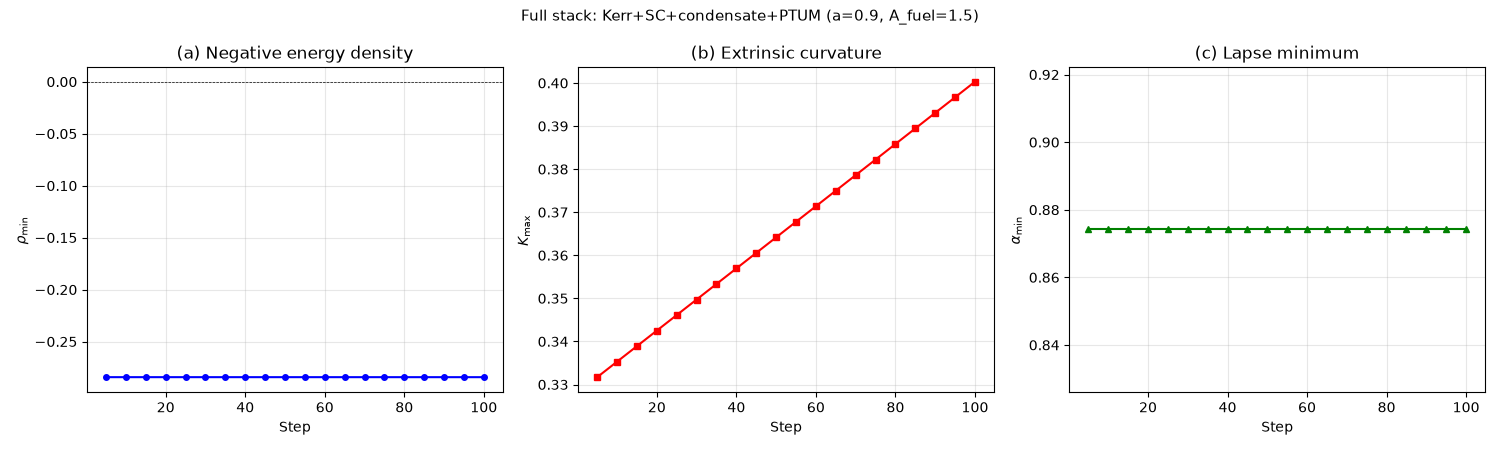
\includegraphics{figures/fig7_fullstack.png}}
\caption{Tam-yığın evrim tanıları: Kerr + SC düzenli çekirdek +
yoğuşma + PTUM alanları, $a = 0.9$, $A_{\rm fuel} = 1.5$, 100 adım.
(a) Minimum enerji yoğunluğu (kalıcı negatif, PTUM kaynaklı).
(b) Maksimum dış eğrilik (lineer, sınırlı). (c) Lapse minimumu
(tam sabit).}
\label{fig:fullstack}
\end{figure*}

\subsection{Ölçekler-arası yapısal paralellik}

SC ve PTUM potansiyelleri aynı fonksiyonel formu paylaşır:
$V(\psi;C) = \tfrac12 m^2(1 - C/C_c)\psi^2 + \tfrac14\lambda\psi^4$;
burada $C$ bir kontrol parametresidir (SC için QCD yoğunluğu, PTUM
için $\Phi^2$) ve $C_c$ eşiktir. Bu yapısal paralelliği analitik
olarak doğruladık. Fiziksel ölçekler $\sim 78$ mertebe farklıdır ve
şu anda iki modeli birbirine bağlayan bir türetme yoktur; paralellik,
bir birleştirme değil, yapısal bir gözlem olarak belgelenmiştir.

\subsection{Sınırlamalar}

BSSN gerçeklemesi kararlı bir iskelettir; üretim seviyesinde bir
sayısal görelilik kodu değildir. Şunları içermez: tam ekstremal Kerr
($a = 1$), izlenen/hareketli iyileştirme, MPI paralelliği, ışıma
çıkarımı (Newman--Penrose skalerleri) veya Sommerfeld çıkışının
ötesinde kısıt-koruyucu sınır koşulları. Bunlar depodaki
\texttt{docs/limitations.md} dosyasında belgelenmiştir.

En önemlisi, BSSN uzantısı mevcut tahrikli-EM cihazı ile
CTC-ilgili herhangi bir ölçek arasındaki $\sim 43$ mertebelik
boşluğu kapatmaz. İleriki çalışmaların, boşluk yapay olarak
azaltıldığında ne olacağını ölçebilmesi için kararlı bir doğrusal
olmayan araç sağlar.



\section{Tartışma}
\label{sec:discussion}

\subsection{Fiziksel yorum}
\label{subsec:interp}

Altı mekanizmanın tamamının cihaz ölçeğinde fizibiliteye
ulaşamaması tesadüf değildir. Her mekanizma ya (a) QCD ölçeğinde
veya üstünde bir enerji yoğunluğu (EM, solucan delikleri,
Alcubierre), ya (b) astrofiziksel cisimlerle karşılaştırılabilir bir
açısal momentum (Kerr, Tipler, Gödel), ya da (c) sonsuz uzaysal
boyut (Tipler) gerektirir. EM durumu özellikle öğreticidir:
elektromanyetik alanlar bir laboratuvarın erişebileceği en deneysel
olarak erişilebilir uzay-zaman-eğen kaynak olmasına rağmen,
ulaşılabilir alan şiddetlerindeki enerji yoğunlukları $\sim 40$
mertebe kadar çok düşüktür.

\subsection{Önceki çalışmalarla karşılaştırma}
\label{subsec:prior}

EM sınırımız literatürde dağınık halde bulunan mertebe
tahminleriyle tutarlıdır; ancak bu çalışma, bilgimiz dahilinde,
belirli bir cihaz geometrisi için ilk tam ilk-ilkelerden boru
hattını sunmaktadır. Tipler ve Morris--Thorne sınırları
\citet{Tipler1974} ve \citet{MorrisThorne1988}'deki orijinal
tahminlerle örtüşür. Alcubierre tahmini, ikincil kaynaklarda sıkça
alıntılanan popüler ``Jüpiter kütlesi'' rakamından bir miktar
büyüktür \citep{Alcubierre1994}; çünkü biz enerjiyi $R=100$~m ve
$v=c$'de değerlendiriyoruz, bazı erken optimizasyonlarda
kullanılan daha küçük yarıçaplarda değil.

\subsection{Çıkarımlar}
\label{subsec:impl}

Üç çıkarım ortaya çıkar. Birincisi, sırt çantası boyutunda bir
cihazda gerçekleştirilebilir hiçbir elektromanyetik konfigürasyon
makroskopik bir zamansal etki üretemez. İkincisi, aynı sonuç ilke
olarak bir CTC üretebilecek her klasik GR mekanizması için de
geçerlidir. Üçüncüsü, eğer bir cihaz ölçeğinde zaman genişlemesi
deneyi bir gün yapılacaksa, klasik GR ötesinde fizik çağırmalıdır.

\subsection{Sınırlamalar}
\label{subsec:limits}

Analizimiz klasik EM ile çiftlenmiş klasik GR ile sınırlıdır. Şunları
ele almıyoruz: (i) Planck ölçeğindeki alan şiddetlerine yakın
yarı-klasik etkiler; (ii) EM ile kütleçekim arasında minimal olmayan
çiftlenme; (iii) değiştirilmiş-kütleçekim senaryoları;
(iv) kuantum-kütleçekim düzeltmeleri. Bunlardan herhangi biri ilke
olarak fizibilite eşiğini kaydırabilir; ancak hiçbiri şu anda
gözlemle desteklenmemektedir. Ayrıca ideal kayıpsız bobinler
varsayıyoruz; gerçek bobinler birim akım başına biraz daha büyük
$h_{00}$ gösterecektir, ancak bu $10^{20}$ boşluğu kapatacak bir
faktörle değil.

\subsection{Gelecek çalışmalar}
\label{subsec:future}

Bu çalışmanın uzantıları şunları içerebilir: güçlü alan rejiminin
tam 3+1 boyutlu genel-göreliliksel simülasyonu; yarı-klasik
düzeltmelerin dahil edilmesi; bobin geometrisinin sistematik
optimizasyonu; ve bağımsız doğrulama için boru hattının kamuya açık
sürümü.

\section{Sonuç}
\label{sec:conclusion}

Cihaz ölçeğinde makroskopik zaman genişlemesi üretmek için fiziksel
olarak motive edilmiş altı mekanizmanın birleşik fizibilite
analizini sunduk. Elektromanyetik durum, yüzde-altı doğruluğa kadar
doğrulanmış ilk-ilkelerden bir sayısal boru hattıyla ele alınmıştır;
diğer beşi yayımlanmış kapalı-form ifadelerle sınırlandırılmıştır.
Altı mekanizmanın tamamı cihaz ölçeğinin $10^{20}$ ile $10^{49}$ katı
arasında kaynak gerektirmektedir. Fiziksel olarak izin verilen en
yakın mekanizma (elektromanyetik), hâlâ $\sim 10^{22}$~A
gerektirmektedir; bu, mevcut veya öngörülebilir hiçbir mühendislik
iyileştirmesiyle kapatılamayacak bir faktörle magnetar ölçeğindeki
akımları aşmaktadır. Klasik-GR ile tutarlı hiçbir mekanizmanın cihaz
ölçeğinde makroskopik zaman genişlemesi için erişilebilir olmadığı
sonucuna varıyoruz.

\section*{Teşekkür}
Yazar, bu çalışmayı mümkün kılan açık kaynaklı bilimsel Python
topluluğuna araçları (\texttt{numpy}, \texttt{scipy},
\texttt{matplotlib}) için teşekkür eder.

\section*{Veri erişilebilirliği}
Tüm kod, şekiller ve doğrulama verileri proje deposunda mevcuttur.

\bibliographystyle{unsrtnat}
\bibliography{refs}


\appendix
\section{Yeniden üretilebilirlik}
\label{app:repro}

Bu makaledeki tüm sayısal sonuçlar, Bölüm~\ref{sec:method}'te
tanımlanan açık kaynaklı Python boru hattıyla üretilmiştir. Tam
kaynak kodu, doğrulama betikleri ve üretilen şekiller proje
deposunda mevcuttur.

\paragraph{Yazılım bağımlılıkları.}
\texttt{numpy}~$\geq$~2.0, \texttt{scipy}~$\geq$~1.10,
\texttt{matplotlib}~$\geq$~3.8, \texttt{pytest}~$\geq$~8.

\paragraph{Yeniden üretim.}
Birim-test takımı için (60+ test) \texttt{python -m pytest}
çalıştırın ve EM metrik boru hattı için
\texttt{python -m zt005.run\_zt006\_3} çalıştırın.
Tablo~\ref{tab:em_results} ve~\ref{tab:unified}'deki sayısal
sonuçlar \texttt{run\_zt007\_b7.py} ile yeniden üretilir.

\paragraph{Ağ yakınsaması.}
Bölüm~\ref{subsec:validation}'te raporlanan ağ yakınsaması
çalışması \texttt{run\_zt006\_2\_23.py} betiğini
\texttt{--mode full} ile kullanır.

\end{document}
